\chapter[Configuración de Eclipse.]{Configuracion del entorno de programación Eclipse.}\label{cap:apendiceA}

A continuación vamos a explicar como instalar y configurar Eclipse para que podamos programar para la plataforma Android y la plataforma Google App Engine, vamos a explicar como instalar los plugins que proporciona Google en ambos casos.

\section{Configuración de Eclipse para Android.}\label{cap:configuracionAndroidEclipse}

Lo primero que tenemos que hacer es descargarnos Eclipse y el SDK de Android. Para el primero vamos a la web \url{http://www.eclipse.org/downloads/} y bajamos la versión classic de Eclipse. Yo recomiendo la versión Eclipse Classic porque es la versión básica que trae todo lo necesario para programar para Android. A continuación bajamos el SDK de Android de la siguiente web \url{http://developer.android.com/sdk/index.html}. Al haber realizado el proyecto en Ubuntu toda esta configuración será para Linux, pero es equivalente a la que debemos realizar en Windows o Mac, al ser todo el software multiplataforma, solo tendríamos que descargar las versiones específicas para nuestro sistema operativo.

Una vez descargados ambos archivos procedemos descomprimirlos, con lo que obtenemos dos carpetas, una con el SDK de Android y otra con Eclipse. A continuación vamos a instalar el SDK de Android, para ello abrimos una terminal y nos desplazamos a la carpeta \textit{\\tools} dentro de la carpeta donde hemos descomprimido el SDK y ejecutamos el siguiente comando: 

\begin{lstlisting}[style=consola]
./android sdk
\end{lstlisting}

El resultado de ejecutar este comando podemos verlo en la figura~\ref{fig:androidSDK}.

\begin{figure}[hbt]
  \centering
    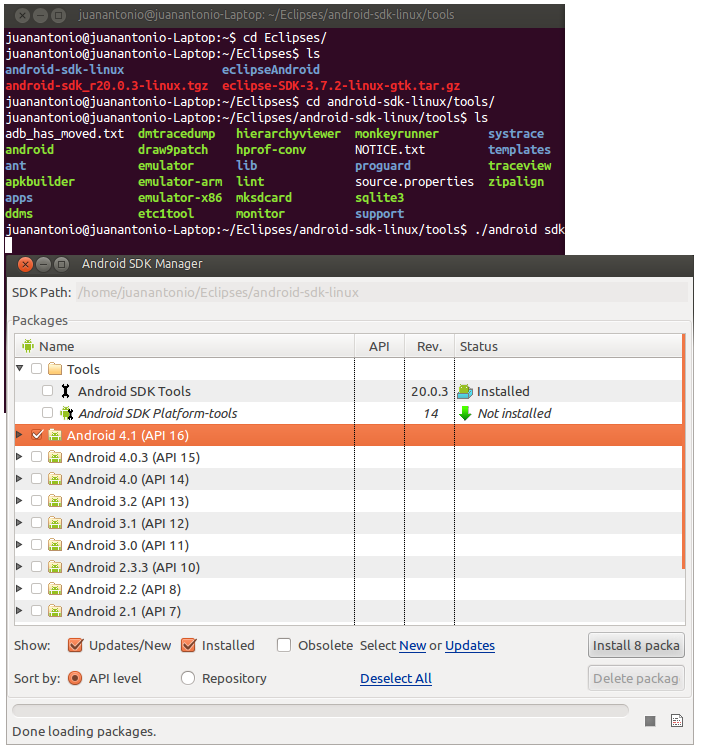
\includegraphics[scale=0.4]{./ConfiguracionEclipse/imagenes/androidSDK.png}
  \caption{Ventana de instalación del SDK de Android.}
  \label{fig:androidSDK}
\end{figure}

En la pantalla que aparece podemos elegir que versión del SDK queremos instalar dependiendo de la versión sobre la que queramos desarrollar, nosotros instalaremos la versión 4.0. Seleccionamos la versión 4.0 y pulsamos en instalar. Aceptamos las licencias y pulsamos en Install (figura~\ref{fig:licencias}), acto seguido el instalador empieza a descargar e instalar todos los paquetes que hemos seleccionado.

\begin{figure}
  \centering
    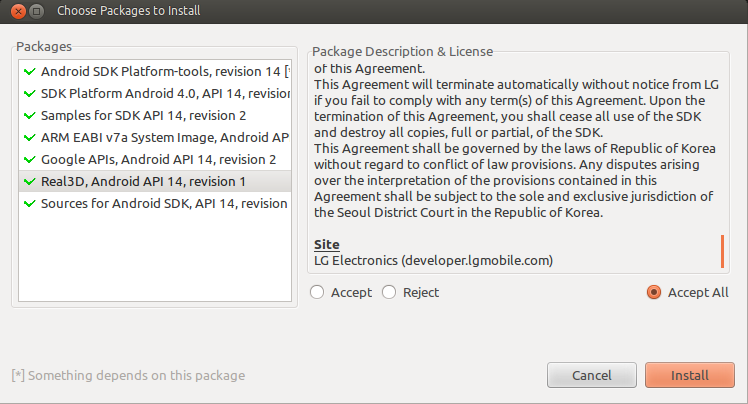
\includegraphics[scale=0.6]{./ConfiguracionEclipse/imagenes/licencias.png}
  \caption{Ventana para aceptar las licencias.}
  \label{fig:licencias}
\end{figure}

\begin{figure}
  \centering
    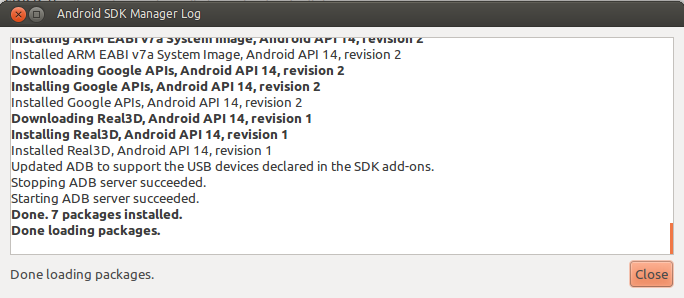
\includegraphics[scale=0.6]{./ConfiguracionEclipse/imagenes/SDKfinalizado.png}
  \caption{Instalación del SDK finalizada.}
  \label{fig:SDKfinalizado}
\end{figure}

Una vez hemos instalado el SDK (figura~\ref{fig:SDKfinalizado}) tenemos que instalar el puglins para Eclipse, para ello abrimos Eclipse y vamos a \textbf{Help}, \textbf{Install New Software}, pulsamos en \textbf{Add} y copiamos la siguiente dirección web, \url{https://dl-ssl.google.com/android/eclipse/} y pulsamos \textbf{Ok}. En la figura~\ref{fig:instalacionADT} podemos ver el resultado y la opción que tenemos que marcar. Pulsamos \textbf{Siguiente} y aceptamos las licencias y pulsamos \textbf{Finalizar}, a continuación Eclipse empezará a descargar los paquetes que le hemos solicitado y cuando termine los instalará.

\begin{figure}
  \centering
    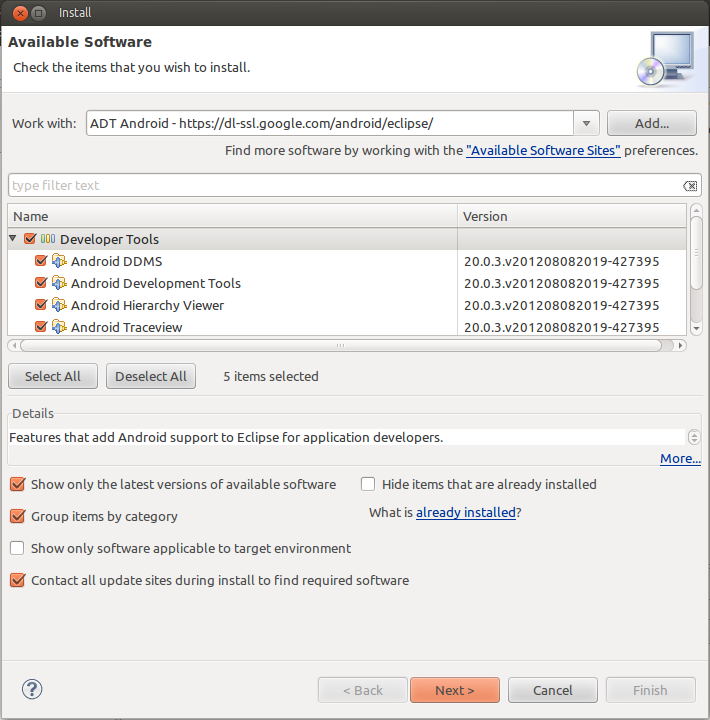
\includegraphics[scale=0.6]{./ConfiguracionEclipse/imagenes/instalacionADT.png}
  \caption{Instalación del ADT en Eclipse.}
  \label{fig:instalacionADT}
\end{figure}

Una vez instalados nos pide que reiniciemos Eclipse, al iniciar de nuevo nos aparecerá un asistente para la configuración del SDK, tendremos que saber la ruta donde lo hemos instalado anteriormente. Podemos ver el asistente en la siguiente figura~\ref{fig:configuracionSDK}.
 
\begin{figure}
  \centering
    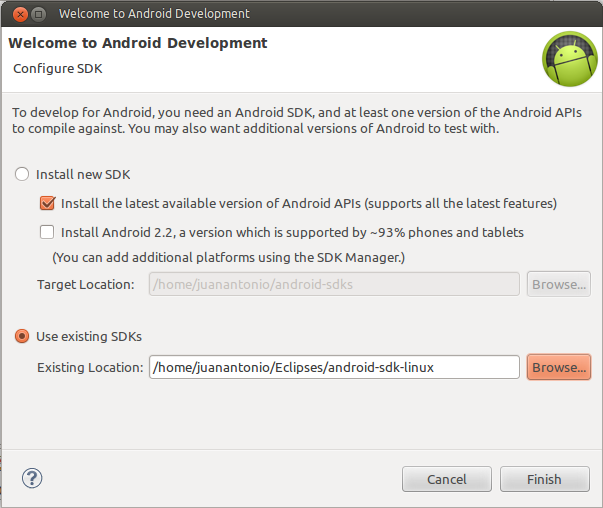
\includegraphics[scale=0.6]{./ConfiguracionEclipse/imagenes/configuracionSDK.png}
  \caption{Instalación del SDK en Eclipse.}
  \label{fig:configuracionSDK}
\end{figure}

Como podemos observar en la figura~\ref{fig:nuevoProyectoAndroid} ya tenemos configurado Eclipse para programar en Android.

\begin{figure}
  \centering
    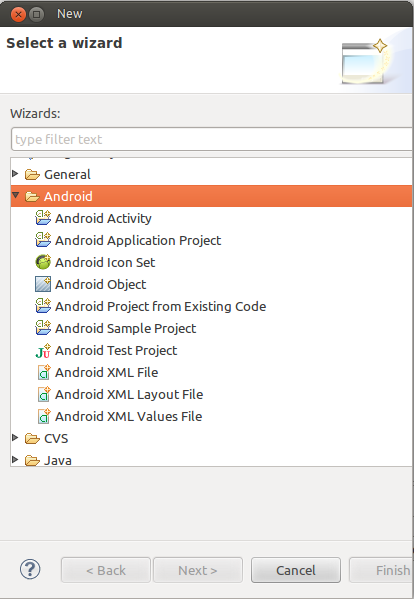
\includegraphics[scale=0.6]{./ConfiguracionEclipse/imagenes/nuevoProyectoAndroid.png}
  \caption{Creación de un nuevo proyecto Android.}
  \label{fig:nuevoProyectoAndroid}
\end{figure}

Para el uso de Git hemos usado el plugins eGit, que se puede descargar gratuitamente de la web \url{http://www.eclipse.org/egit/}. En dicha web también podemos ver la forma de instalación y configuración, que es muy sencilla y solo se necesita la URL del servidor, el nombre de usuario y el password.

\section{Configuración de Eclipse para Google App Engine.}\label{cap:configuracionGAEEclipse}

Al igual que en el apéndice~\ref{cap:configuracionAndroidEclipse} necesitamos tener una versión de Eclipse Classic, yo recomiendo tener un Eclipse diferente para cada plugins que queramos utilizar, así evitamos incompatibilidades entre ellos. Comenzamos como en la instalación del ADT para Eclipse, abriendo Eclipse y pulsamos en \textbf{Help}, \textbf{Install New Software}, luego en \textbf{Add} y copiamos la siguiente dirección web, \url{http://dl.google.com/eclipse/plugin/3.7} y pulsamos \textbf{Ok}. En la figura~\ref{fig:instalacionGAE} podemos ver el resultado y los paquetes que nos da la posibilidad de instalar.

\begin{figure}[hbt]
  \centering
    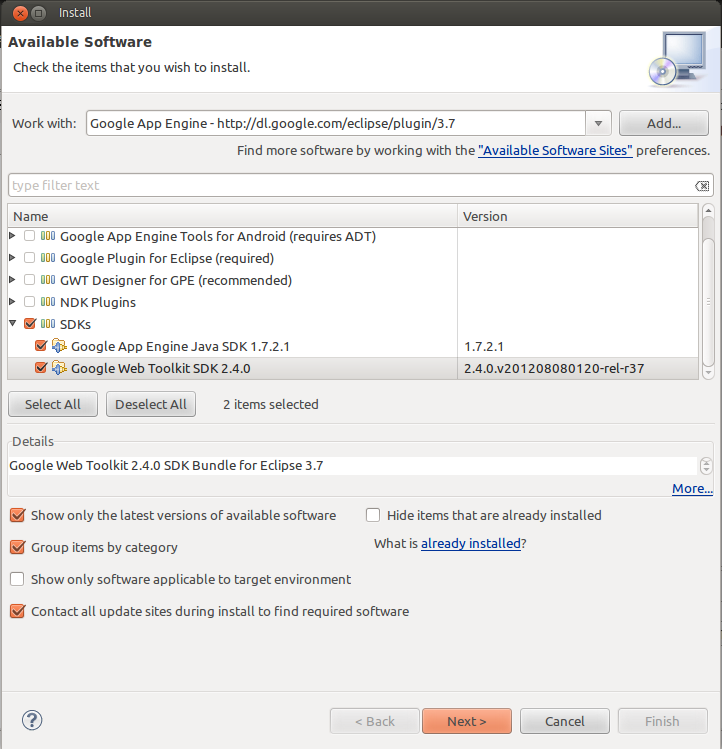
\includegraphics[scale=0.6]{./ConfiguracionEclipse/imagenes/instalacionGAE.png}
  \caption{Instalación puglins Google App Engine.}
  \label{fig:instalacionGAE}
\end{figure}

A nosotros nos interesa el paquete que está dentro de \textbf{SDK}, \textbf{Google App Engine Java SDK}, también necesitamos el \textbf{Google Plugin for Eclipse 3.7} y si queremos hacer diseño de la interfaz web de la aplicación podemos instalar \textbf{GWT Designer for GPE}, nosotros no lo usaremos en el proyecto. A continuación pulsamos \textbf{Siguiente}, aceptamos las licencias y pulsamos \textbf{Finalizar}. Acto seguido Eclipse empezará a descargar los plugins y a instalarlos (figura~\ref{fig:instalacionPlugins}), cuando termine nos pedirá que reiniciemos Eclipse.

\begin{figure}[hbt]
  \centering
    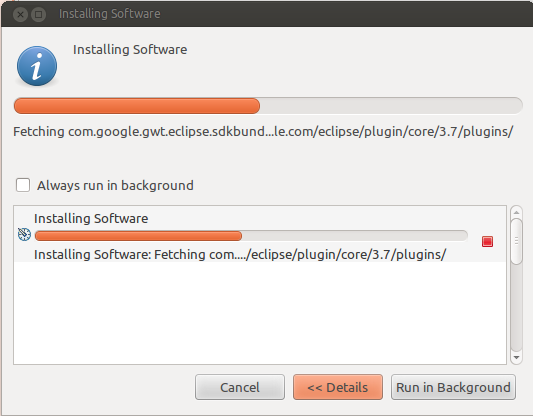
\includegraphics[scale=0.6]{./ConfiguracionEclipse/imagenes/instalacionPlugins.png}
  \caption{Detalle de la descarga de plugins.}
  \label{fig:instalacionPlugins}
\end{figure}

Cuando se vuelve a abrir Eclipse ya vemos que hay varias cosas que han cambiado como podemos ver en la figura~\ref{fig:eclipseGAE}. Podemos ver que ya estamos logueados con nuestra cuenta de usuario y nos da la posibilidad de crear aplicaciones web en la plataforma. En el botón de Google también hay una acción muy importante que explicaremos posteriormente que es la de desplegar una aplicación web en el servicio de Google App Engine. Todo lo que hagamos podemos probarlo en local simplemente pulsado el botón play y Eclipse deplegará un servidor Tomcat en el que probar la aplicación web que desarrollemos.

\begin{figure}[hbt]
  \centering
    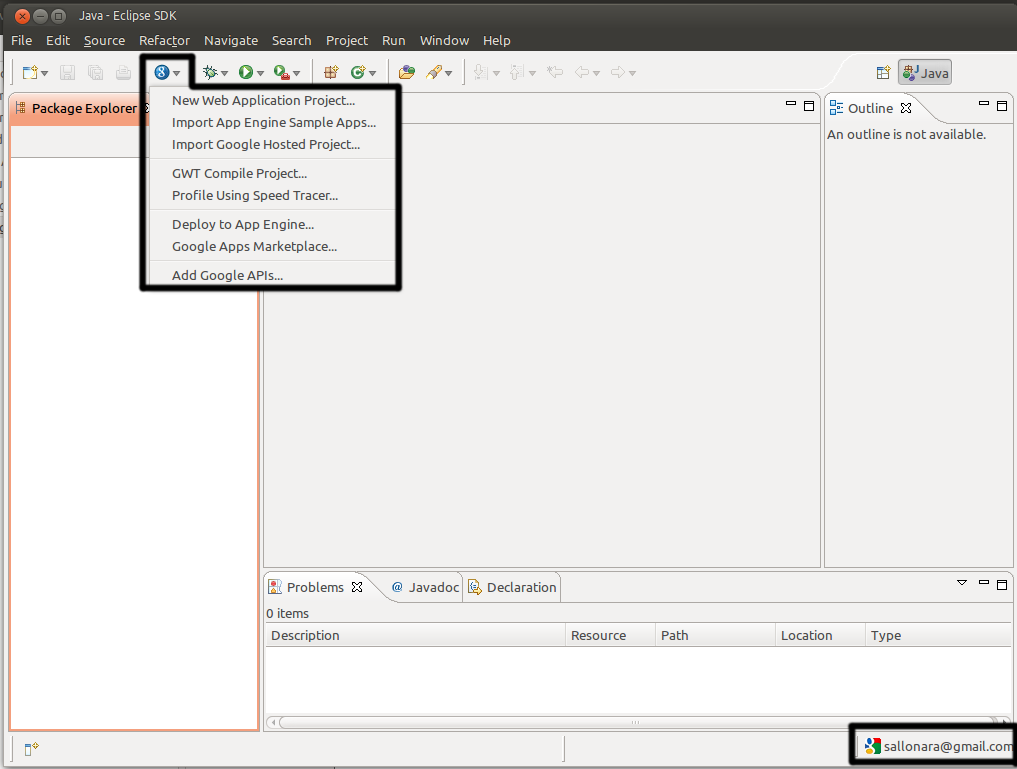
\includegraphics[scale=0.5]{./ConfiguracionEclipse/imagenes/eclipseGAE.png}
  \caption{Eclipse con el plugin de Google App Engine instalado.}
  \label{fig:eclipseGAE}
\end{figure}

Una vez preparado Eclipse para que podamos programar, hay que genera los dominios donde correrán nuestras aplicaciones web. De forma gratuita Google proporciona 10 dominios diferentes por cuenta. Para crearlos hay que ir a la siguiente dirección web: \url{https://appengine.google.com/}, en ella nos logueamos con nuestra cuenta de Google, podemos ver en la figura~\ref{fig:appEngine} el panel de administración de las aplicaciones.  

\begin{figure}[hbt]
  \centering
    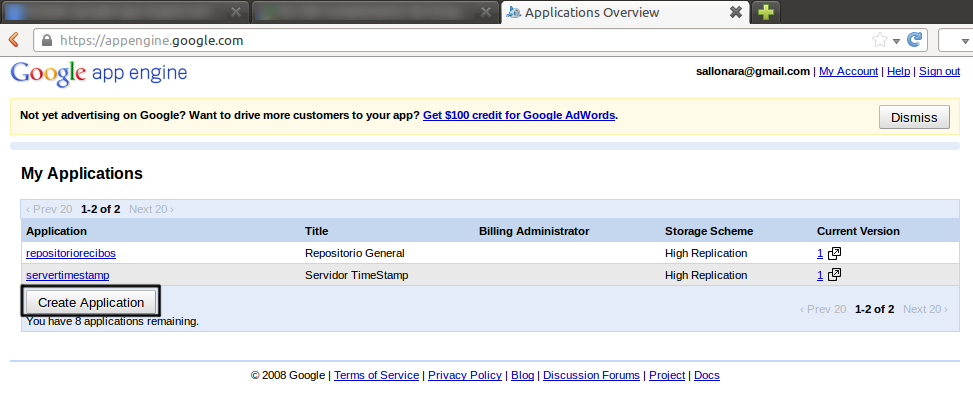
\includegraphics[scale=0.6]{./ConfiguracionEclipse/imagenes/appEngine.png}
  \caption{Panel de administración Google App Engine.}
  \label{fig:appEngine}
\end{figure}

Pulsando el botón \textbf{Create Application} tenemos acceso a todos los parámetros de configuración para la aplicación web. En la imagen~\ref{fig:createGAE} podemos ver los parámetros que nos pide, vemos que no son muchos, un nombre que será el dominio que nos proporcionará Google, el título de la aplicación web y la forma de logueo que queremos que tenga nuestra aplicación en caso de necesitarla.

\begin{figure}[hbt]
  \centering
    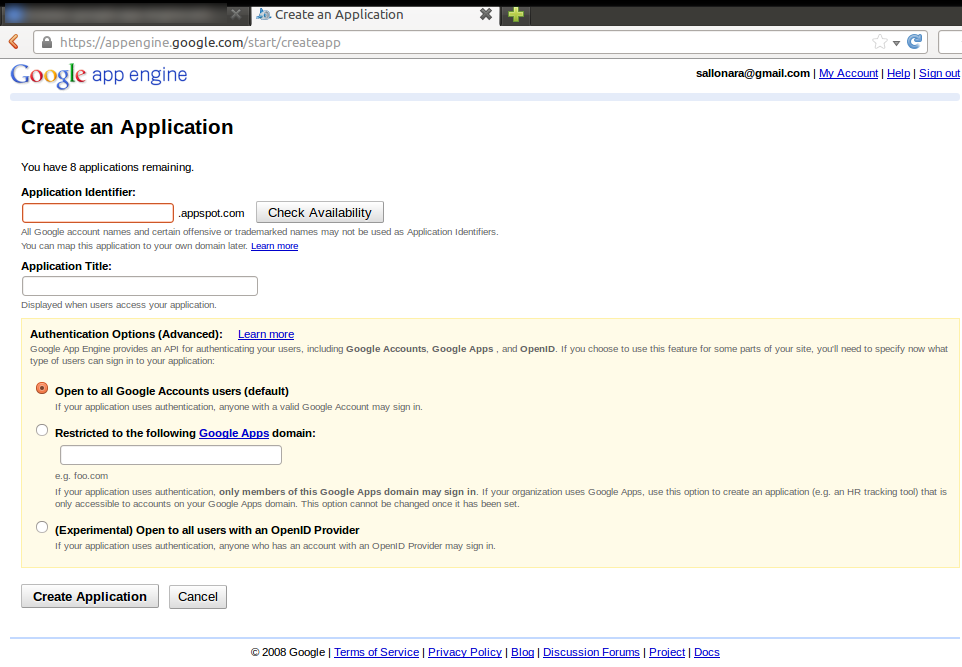
\includegraphics[scale=0.5]{./ConfiguracionEclipse/imagenes/createGAE.png}
  \caption{Parámetros para la creación de una nueva aplicación web.}
  \label{fig:createGAE}
\end{figure}

Una vez creada la aplicación web, tenemos acceso a un dashboard donde podemos configurar otras opciones de la aplicación, ver estadísticas, los log, administrar la base de datos, etc. Podemos verlo en la figura~\ref{fig:dashboardGAE}.

\begin{figure}[hbt]
  \centering
    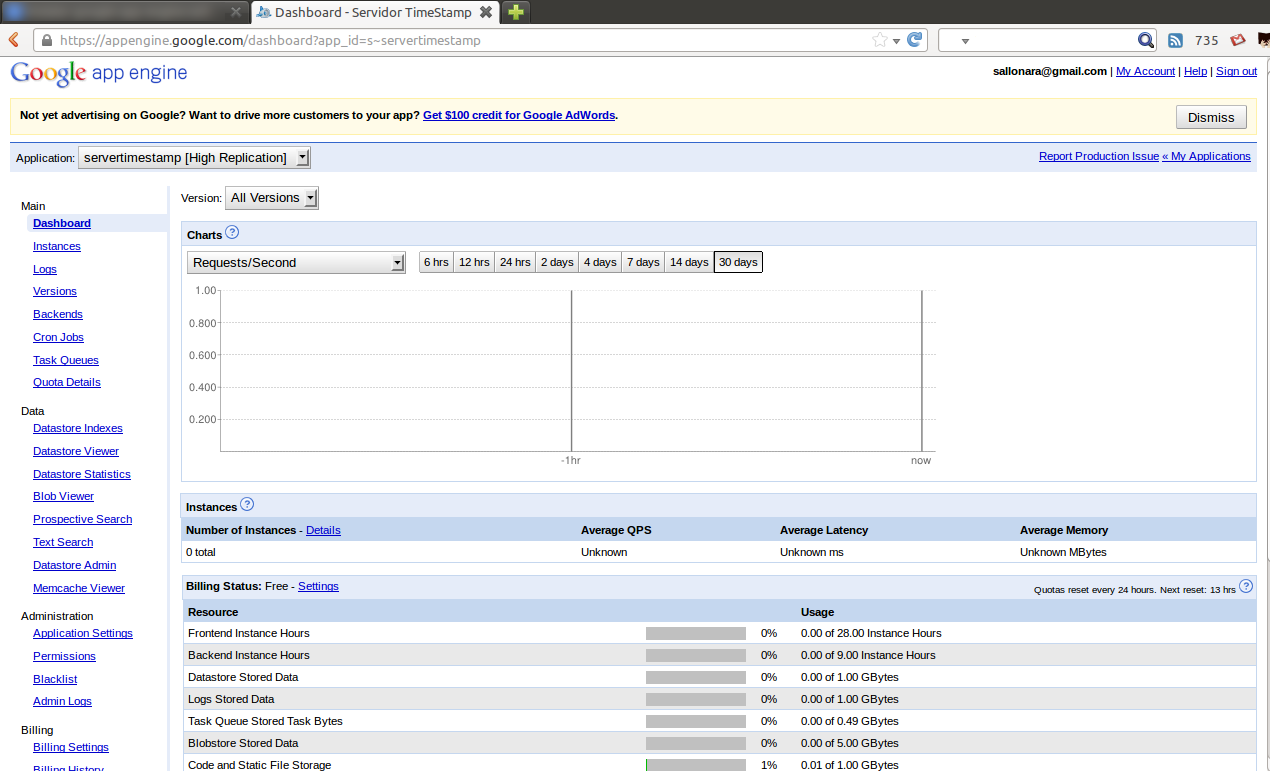
\includegraphics[scale=0.4]{./ConfiguracionEclipse/imagenes/dashboardGAE.png}
  \caption{Dashboard para la configuración de una aplicación web.}
  \label{fig:dashboardGAE}
\end{figure}

Con esto habríamos terminado la parte de la creación de la aplicación web y a continuación vamos a explicar como hacer el despliegue de una aplicación con Eclipse.

Una vez tenemos un proyecto creado y testeado procederemos a la subida, para eso tendríamos que pulsar en el botón de Google que vimos antes y pulsar en la opción \textbf{Deploy to App Engine}. Nos aparece una nueva ventana en la que debemos configurar unos parámetros básicos, pero si es la primera vez que vamos a hacer el despliegue tenemos pulsar en \textbf{App Engine project settings...} (figura~\ref{fig:GAESettings}), en la ventana que nos aparece podemos configurar muchos más parámetros, el más importante el \textbf{Application ID} y \textbf{Version}. En \textbf{Application ID} tenemos que poner el nombre con el que hemos creado la aplicación web, en nuestro caso \textit{repositoriorecibos}. También podemos cambiar la versión del SDK que queremos usar, que según hemos podido observar durante el desarrollo del proyecto se ha actualizado varias veces, si la base de datos es altamente replicada, etc.

\begin{figure}[hbt]
  \centering
    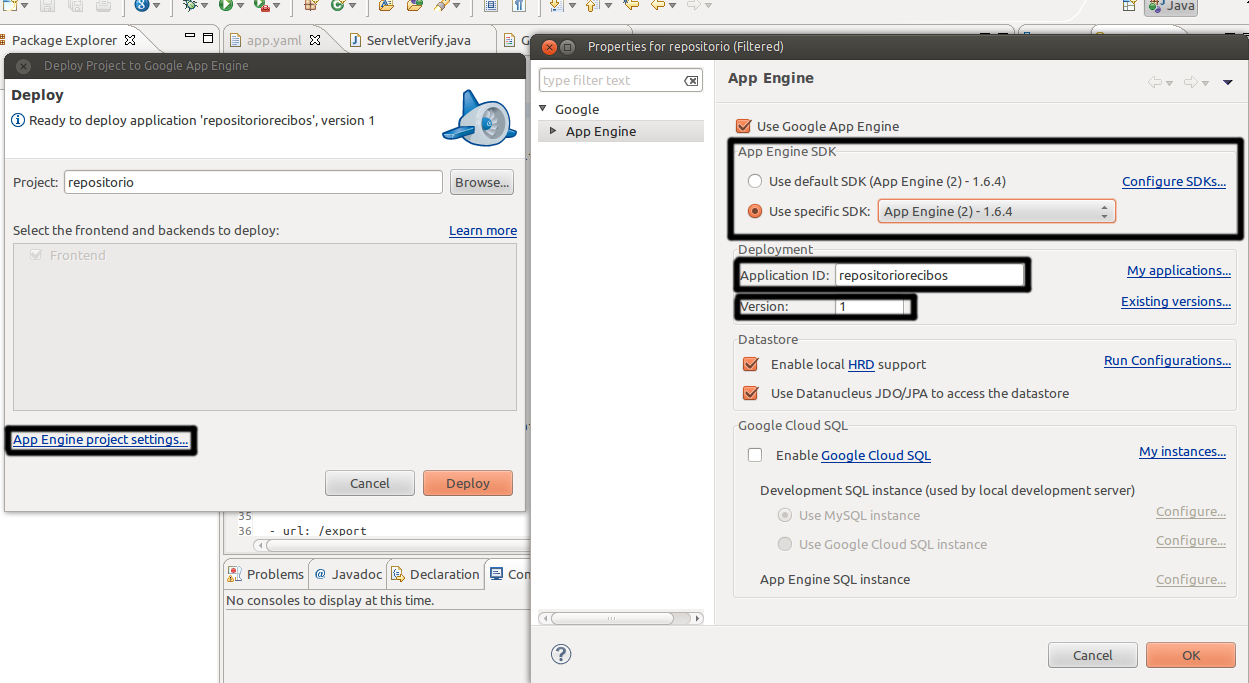
\includegraphics[scale=0.4]{./ConfiguracionEclipse/imagenes/GAESettings.png}
  \caption{Despliegue de una aplicación web.}
  \label{fig:GAESettings}
\end{figure}

Una vez realizado el despliegue ya podemos tener acceso a la aplicación web mediante el link \url{http://nombre\_aplicacion.appspot.com}.

